\chapter[Testy i eksperymenty]{Testy i eksperymenty}

\label{chapter:testy}

\section{Test przetwornika piezoelektrycznego}
Pierwszym testem był test przetwornika, który jest nadajnikiem sygnału. Zasilono go bezpośrednio z generatora wbudowanego w oscyloskop, 
parametry zadane to sygnał sinusoidalny o napięciu \unit[5]{V} \textit{peak-to-peak} czyli wartości szczytowej.
Elementem odbiorczym był inny przetwornik piezoelektryczny służący tylko do testów, został on umieszczony w odległości \unit[10]{cm} od nadajnika. 
Jego częstotliwość rezonansowa również wynosiła \unit[40]{kHz}.
Po podłączeniu sondy oscyloskopu do odbiornika ukazał się bardzo wyraźny sygnał w kształcie sinusoidy ustawionej na nadajniku.
Dźwięki otoczenia miały bardzo znikomy wpływ na zakłócenia, stanowiąc niewielki procent amplitudy. 
Zmiana częstotliwości o chociażby \unit[1]{kHz} wiązała się kilkudziesięciokrotnym spadkiem mocy sygnału, co potwierdzało dane z noty katalogowej elementu piezoelektrycznego.
\begin{figure}[!ht]
    \centering
    \missingfigure{screen z oscylo z przebiegiem sygnału z piezo}
    \caption{Przebieg sygnału odebrany innym przetwornikiem piezoelektrycznym}
    \label{fig:oscylo_piezo}
\end{figure}

\section{Test wpływu odległości na sygnał}
Z identycznym stanowiskiem pomiarowym co sekcję wyżej sprawdzono wpływ odległości czujników na moc i przesuniecie fazy sygnału.
Zmieniając odległość nadajnika od odbiornika dało się w czasie rzeczywistym wyraźnie zauważyć przesuwanie sie fazy sygnału jak i jego amplitudę. 
\todo{zdjęcie z oscylo z przesuniętym sygnałem i kilka testów na różne odległości}

\begin{figure}[!ht]
    \centering
    \missingfigure{screen z oscylo z przebiegiem sygnału z piezo}
    \caption{Przebieg sygnału odebrany innym przetwornikiem piezoelektrycznym, wpływ na odległość}
    \label{fig:oscylo_piezo2}
\end{figure}

\section{Pierwsze uruchomienie}
PCB z przylutowanymi elementami zostało podłączone do zasilacza laboratoryjnego dostarczającego \unit[5]{V} i ograniczeniem prądowym ustawionym na \unit[100]{mA}. 
Pierwsze uruchomienie sterownika\todo{???} sonaru ujawniło drobny błąd projektowy, wszystkie diody elektroluminoescencyjne zostały przylutowane w złej polaryzacji.
Szybka zmiana ustawień diod i następne uruchomienie, nie pokazywało oznak większych błędów. Pobór prądu wyniósł\todo{podać ile prądu ciągnie}, a temperatura elementów na 
płytce nie odstawała od temperatury pokojowej.

\section{Uruchomienie i test wzmacniacza sygnału przetwornika piezoelektrycznego}
Wzmacniacz nadajnika zachował się zgodnie z założeniami projektowymi, na wyjściu otrzymane zostało \unit[80]{V} peak-to-peak. 

\begin{figure}[!ht]
    \centering
    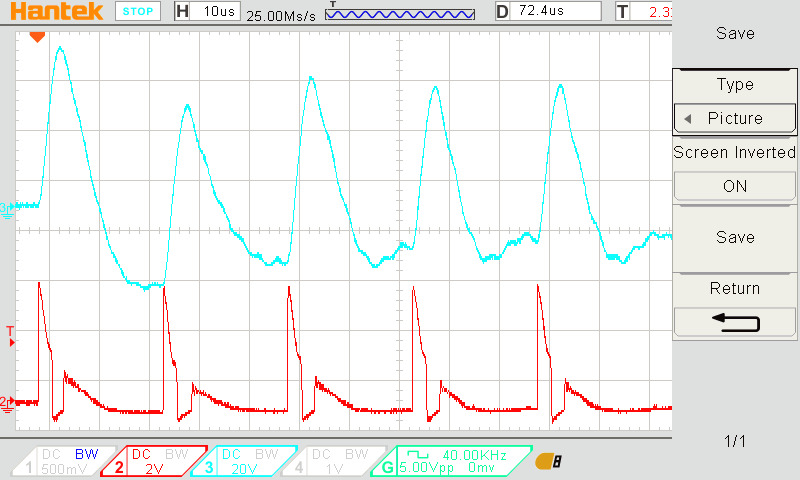
\includegraphics[width = 0.5\textwidth]{piezo_oscylo.jpg}
    \caption{Wyjście transformatora z podłączonym przetwornikiem piezoelektrycznym}
    \label{fig:oscylo_piezo3}
\end{figure}

\section{Test mikrofonów i filtrów}
Test miał na celu sprawdzenie jaki poziom sygnału dostarczają same mikrofony oraz na 

\begin{figure}[!ht]
    \centering
    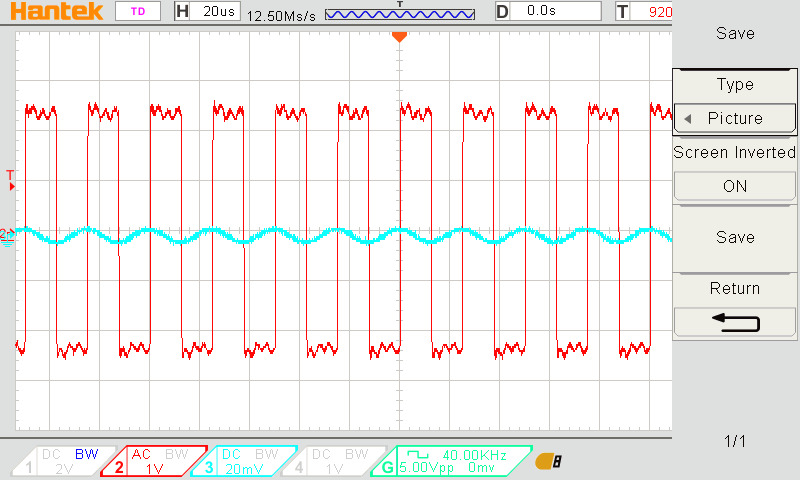
\includegraphics[width = 0.5\textwidth]{microphone.jpg}
    \caption{Przebieg sygnału odebrany bezpośrednio przez mikrofon MEMS}
    \label{fig:oscylo_piezo4}
\end{figure}

\begin{figure}[!ht]
    \centering
    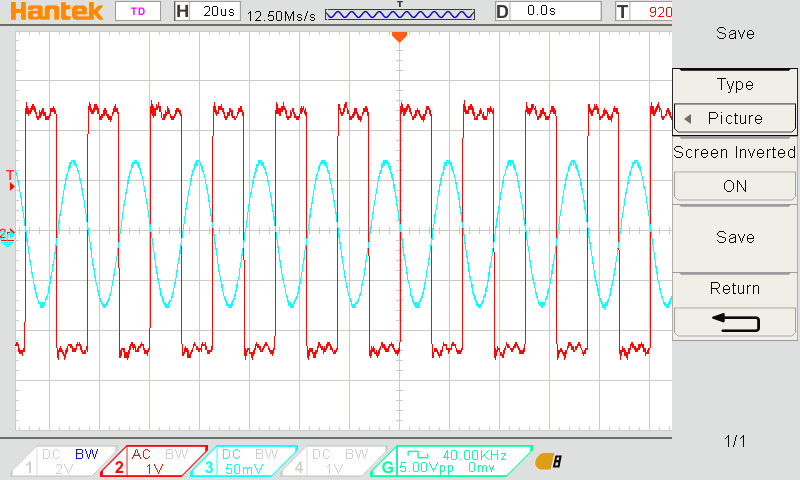
\includegraphics[width = 0.5\textwidth]{filter.jpg}
    \caption{Przebieg sygnału odebrany bezpośrednio przez mikrofon MEMS}
    \label{fig:oscylo_piezo4}
\end{figure}
